\begin{name}
	{ÔN TẬP KIỂM TRA CUỐI HỌC KÌ 1 - KNTT}
	{TOÁN 10}
	{LỚP TOÁN THẦY PHÁT}
	{\thoigian}
\end{name}

%================================PHẦN I
\caulc
\Opensolutionfile{ans}[ans/0-HK1-KN-3-DoanThiDiem-HaNoi-2324-Phan-I]

\begin{ex}%[0-HK1-KN-3-DoanThiDiem-HaNoi-2324]%[VN-MT-6,VM032]%[0D1N3-3]
	Cho tập hợp $A=(-1;2)$; $B= [0;3]$. Khi đó, tập $A\cap B$ là
	\choice
	{\True $ [ 0;2)$}
	{$ (-1;3]$}
	{$ (-1;0)$}
	{$ [2;3]$}
	\loigiai{
		\begin{center}
			\begin{tikzpicture}[scale=1, font=\footnotesize, line join=round, line cap=round, >=stealth]
				\draw[-stealth] (-2,0)--(4,0);
				\path 
				(-1,0)node{$($} +(90:0.5) node{$-1$}
				(2,0) node{$)$} +(90:.5) node{$2$}
				(0,0) node{$[$} +(90:.5) node{$0$}
				(3,0) node{$]$} +(90:.5) node{$3$}
				; 
				\fill[opacity=0.6,pattern=north east lines] (-2,-4pt) rectangle (-1,4pt) (2,-4pt) rectangle (3.9,4pt);
				\fill[opacity=0.6,pattern=north west lines] (-2,-4pt) rectangle (0,4pt) (3,-4pt) rectangle (3.9,4pt);
			\end{tikzpicture}
		\end{center}
		Ta có $A\cap B=(-1;2)\cap [0;3]=[0;2)$.}
\end{ex}


\begin{ex}%[0-HK1-KN-3-DoanThiDiem-HaNoi-2324]%[VN-MT-6,VM032]%[0H9N2-1]
	Trong mặt phẳng tọa độ $Oxy$, cho các vectơ $\overrightarrow{u}=( 5;-3 ),$$\overrightarrow{v}=( 1;2 )$. Tích vô hướng của hai vectơ $\overrightarrow{u}$ và $\overrightarrow{v}$ là
	\choice
	{\True $\overrightarrow{u}\cdot \overrightarrow{v}=-1$}
	{$\overrightarrow{u}\cdot \overrightarrow{v}=-13$}
	{$\overrightarrow{u}\cdot \overrightarrow{v}=0$}
	{$\overrightarrow{u}\cdot \overrightarrow{v}=5$}
	\loigiai{Tích vô hướng của hai vectơ $\overrightarrow{u}$ và $\overrightarrow{v}$ là $\overrightarrow{u}\cdot \overrightarrow{v}=5\cdot 1+(-3)\cdot 2 = -1$.}
\end{ex}

\begin{ex}%[0-HK1-KN-3-DoanThiDiem-HaNoi-2324]%[VN-MT-6,VM032]%[0D6N1-1]
	Cho số đúng $\overline{a}=2{,}85$ và số gần đúng $a=2{,}8$. Sai số tuyệt đối của số gần đúng $a$ là
	\choice
	{$0{,}5$}
	{$0{,}01$}
	{$0{,}1$}
	{\True $0{,}05$}
	\loigiai{Sai số tuyệt đối của số gần đúng $a$ là $\Delta a=\left|\overline{a}-a\right|=0{,}05$.}
\end{ex}

\begin{ex}%[0-HK1-KN-3-DoanThiDiem-HaNoi-2324]%[VN-MT-6,VM032]%[0H4N2-2]
	Cho tam giác $ABC$ có $AB=4$\,cm; $AC=6$\,cm; $\widehat{A}=60^\circ$. Diện tích tam giác $ABC$ là
	\choice
	{\True $6\sqrt{3}$\,cm$^2$}
	{$12\sqrt{3}$\,cm$^2$}
	{$6$\,cm$^2$}
	{$12$\,cm$^2$}
	\loigiai{Ta có $S_{ABC}=\dfrac{1}{2}\cdot AB\cdot AC\cdot \sin A=6\sqrt{3}$\,(cm$^2$).}
\end{ex}

\begin{ex}%[0-HK1-KN-3-DoanThiDiem-HaNoi-2324]%[VN-MT-6,VM032]%[0H5N2-1]
	Cho ba điểm phân biệt $M$; $N$; $P$. Khi đó $\overrightarrow{MN}+\overrightarrow{N}$ bằng
	\choice
	{$\overrightarrow{0}$}
	{\True $\overrightarrow{MP}$}
	{$\overrightarrow{PN}$}
	{$\overrightarrow{PM}$}
	\loigiai{Ta có $\overrightarrow{MN}+\overrightarrow{NP}=\overrightarrow{NP}$.}
\end{ex}

\begin{ex}%[0-HK1-KN-3-DoanThiDiem-HaNoi-2324]%[VN-MT-6,VM032]%[0H9H1-3]
	Trong mặt phẳng tọa độ $Oxy$, cho điểm $M (-3;1)$; $N (0;-1)$. Tọa độ của vectơ $\overrightarrow{MN}$ là
	\choice
	{\True $\overrightarrow{MN}=( 3;-2 )$}
	{$\overrightarrow{MN}=( -2;0 )$}
	{$\overrightarrow{MN}=( 3;0 )$}
	{$\overrightarrow{MN}=( -3;2)$}
	\loigiai{Toạ độ của vectơ $\overrightarrow{MN}$ là $\big(0-(-3);(-1)-1\big)$, hay là $\overrightarrow{MN}=(3;-2)$.}
\end{ex}

\begin{ex}%[0-HK1-KN-3-DoanThiDiem-HaNoi-2324]%[VN-MT-6,VM032]%[0H5H4-1]
	Cho hình vuông $ABCD$. Số đo góc giữa hai vectơ $\overrightarrow{AB}$ và $\overrightarrow{AC}$ bằng 
	\choice
	{$\left( \overrightarrow{AB},\overrightarrow{AC} \right)=30^\circ$}
	{$\left( \overrightarrow{AB},\overrightarrow{AC} \right)=60^\circ$}
	{\True $\left( \overrightarrow{AB},\overrightarrow{AC} \right)=45^\circ$}
	{$\left( \overrightarrow{AB},\overrightarrow{AC} \right)=90^\circ$}
	\loigiai{\begin{center}
			\begin{tikzpicture}[scale=1, font=\footnotesize, line join=round, line cap=round, >=stealth]
				\path 
				(4,0) coordinate (C)
				(4,4) coordinate (B)
				(0,4) coordinate (A)
				(0,0) coordinate (D)
				;
				\draw (B)--(C)--(D)--(A);
				\draw[->] (A)--(B);
				\draw[->] (A)--(C);
				\foreach \x/\g in {A/135,B/45,C/-45,D/-135}
				\fill (\x) circle (1pt) node[shift=(\g:3mm)] {$\x$};
				\draw pic[draw,angle radius=5mm] {angle = C--A--B};
			\end{tikzpicture}
		\end{center}
		Ta có $\left(\overrightarrow{AB},\overrightarrow{AC}\right)=\widehat{BAC}=45^\circ$. Vậy số đo góc giữa hai vectơ $\overrightarrow{AB}$ và $\overrightarrow{AC}$ bằng $45^\circ$. }
\end{ex}


\begin{ex}%[0-HK1-KN-3-DoanThiDiem-HaNoi-2324]%[VN-MT-6,VM032]%[0D1H1-5]
	Phủ định của mệnh đề \lq\lq$\exists x\in \mathbb{R},x^2-2x=0$\rq\rq là mệnh đề nào sau đây?
	\choice
	{\lq\lq$\forall x\in \mathbb{R},x^2-2x=0$\rq\rq}
	{\lq\lq$\exists x\in \mathbb{R},x^2-2x\neq 0$\rq\rq}
	{\True \lq\lq$\forall x\in \mathbb{R},x^2-2x\neq 0$\rq\rq}
	{\lq\lq$\exists x\in \mathbb{R},x^2-2x>0$\rq\rq}
	\loigiai{Phủ định của mệnh đề \lq\lq$\exists x\in \mathbb{R},x^2-2x=0$\rq\rq là mệnh đề \lq\lq$\forall x\in \mathbb{R},x^2-2x\neq 0$\rq\rq.}
\end{ex}

\begin{ex}%[0-HK1-KN-3-DoanThiDiem-HaNoi-2324]%[VN-MT-6,VM032]%[0H4H2-1]
	Cho $\triangle ABC$ có $a=6$, $\widehat{B}=45^\circ$, $\widehat{C}=75^\circ$. Độ dài bán kính đường tròn ngoại tiếp $R$ của tam giác trên là
	\choice
	{\True $R=2\sqrt{3}$}
	{$R=4\sqrt{3}$}
	{$R=6$}
	{$R=12$}
	\loigiai{Do $\widehat{B}=45^\circ$, $\widehat{C}=75^\circ$ nên $\widehat{A}=180^\circ -\widehat{B}-\widehat{C}=60^\circ$.\\
		Áp dụng định lý sin, ta có $R=\dfrac{a}{2\sin A}=\dfrac{6}{2\sin 60^\circ}=2\sqrt{3}$.}
\end{ex}

\begin{ex}%[0-HK1-KN-3-DoanThiDiem-HaNoi-2324]%[VN-MT-6,VM032]%[0D6H1-3]
	Cho số gần đúng $a=678\,356$ với độ chính xác $d=100$. Số quy tròn của số gần đúng $a$ là
	\choice
	{\True $678\,000$}
	{$678\,400$}
	{$679\,000$}
	{$678\,360$}
	\loigiai{Do $d$ là số tự nhiên có $3$ chữ số nên ta sẽ quy tròn $a$ tới hàng nghìn. Vậy số quy tròn của số gần đúng $a$ là $678\,000$.}
\end{ex}

\begin{ex}%[0-HK1-KN-3-DoanThiDiem-HaNoi-2324]%[VN-MT-6,VM032]%[0H5H4-1]
	Cho tam giác $ABC$ đều cạnh $a$. Khi đó, $\overrightarrow{BA}\cdot \overrightarrow{BC}$ bằng
	\choice
	{$a^2$}
	{$a^2\sqrt{3}$}
	{$\dfrac{\sqrt{3}}{2}a^2$}
	{\True $\dfrac{1}{2}a^2$}
	\loigiai{\begin{center}
			\begin{tikzpicture}[scale=1, font=\footnotesize, line join=round, line cap=round, >=stealth]
				\path 
				(0,0) coordinate (B)
				(4,0) coordinate (C)
				(2,{2*sqrt(3)}) coordinate (A)
				;
				\draw (A)--(C);
				\draw[->] (B)--(A);
				\draw[->] (B)--(C);
				\foreach \x/\g in {A/90,B/-120,C/-3}
				\fill (\x) circle (1pt) node[shift=(\g:3mm)] {$\x$};
				\draw pic[draw,angle radius=5mm] {angle = C--B--A};
			\end{tikzpicture}
		\end{center}
		Ta có $\overrightarrow{BA}\cdot \overrightarrow{BC}=\left|\overrightarrow{BA}\right|\cdot \left|\overrightarrow{BC}\right|\cdot \cos \left(\overrightarrow{BA},\overrightarrow{BC}\right)=BC\cdot BC\cdot \cos \widehat{ABC}= a\cdot a\cdot \cos 60^\circ=\dfrac{1}{2}a^2$.}
\end{ex}


\begin{ex}%[0-HK1-KN-3-DoanThiDiem-HaNoi-2324]%[VN-MT-6,VM032]%[0D6H3-3]
	Điểm kiểm tra môn Toán của $9$ học sinh trong một tổ được cho như sau
	\begin{center}
		\begin{tabular}{ccccccccc} 
			$9$&$5$&$7$&$7$&$10$&$6$&$6$&$1$&$8$
		\end{tabular}
	\end{center}
	Tìm trung vị $M_e$ của mẫu số liệu này.
	\choice
	{\True $M_e=5$}
	{$M_e=6$}
	{$M_e=7$}
	{$M_e=6{,}5$}
	\loigiai{Sắp xếp mẫu số liệu theo thứ tự không giảm
		\begin{center}
			\begin{tabular}{ccccccccc} 
				$1$&$5$&$6$&$6$&$\fbox{7}$&$7$&$8$&$9$&$10$
			\end{tabular}
		\end{center}
		Trung vị của mẫu số liệu là $M_e=7$.
	}
\end{ex}
\Closesolutionfile{ans}
%================================PHẦN II
\cauds
\Opensolutionfile{ans}[ans/0-HK1-KN-3-DoanThiDiem-HaNoi-2324-Phan-II]
\setcounter{ex}{0}

\begin{ex}%[0-HK1-KN-3-DoanThiDiem-HaNoi-2324]%[VN-MT-6,VM032]%[0D1V1-2]
	Cho $x$, $k$ là số thực, $n$ là số tự nhiên, $m$ là số hữu tỷ.
	\choiceTF
	{$\forall x\in \mathbb{R},x<2\Leftrightarrow x^2<4$}
	{$\exists k\in \mathbb{R},k^2+1\leq 0$}
	{$\exists m\in \mathbb{Q},m^2-2=0$}
	{\True $\forall n\in \mathbb{N},\left( n^3-n \right)\ \vdots \ 6$}
	\loigiai{
		\begin{itemchoice}
			\itemch \textbf{Sai.}\\
			Chọn $x=-3$, ta có $x<2$ nhưng $x^2=9>4$ (vô lý).
			\itemch \textbf{Sai.} \\
			Ta có $\forall k\in \mathbb{R}$, $k^2\geq 0$ nên $k^2+1\geq 1>0$. Vậy $\nexists k \in \mathbb{R}, k^2+1\leq 0$.
			\itemch \textbf{Sai.} \\
			Xét phương trình $m^2-2=0$. Phương trình có hai nghiệm thực $\hoac{&m=\sqrt{2}\\&m=-\sqrt{2}}$ đều không phải là số hữu tỷ.
			\itemch \textbf{Đúng.} \\
			Ta có $N=n^3-n=(n-1)n(n+1)$ là ba số tự nhiên liên tiếp.\\
			Ta chứng minh $N$ chia hết cho $2$. Thật vậy, ta có các trường hợp
			\begin{itemize}
				\item Nếu $n=2m$, $m \in \mathbb{N}$ thì $N=(2m-1)2m(2m+1)=2\left[(2m-1)m(2m+1)\right] \ \vdots\ 2$.
				\item Nếu $n=2m+1$, $m \in \mathbb{N}$ thì $N=2m(2m+1)(2m+2)=2\left[m(2m+1)(2m+2)\right] \ \vdots\ 2$.
			\end{itemize}
			Vậy $N \ \vdots \ 2$.\\
			Ta chứng minh $N$ chia hết cho $3$. Thật vậy, ta có các trường hợp
			\begin{itemize}
				\item Nếu $n=3m$, $m \in \mathbb{N}$ thì $N=(3m-1)3m(3m+1)=3\left[(3m-1)m(3m+1)\right] \ \vdots\ 3$.
				\item Nếu $n=3m+1$, $m \in \mathbb{N}$ thì $N=3m(3m+1)(3m+2)=3\left[m(3m+1)(3m+2)\right] \ \vdots\ 3$.
				\item Nếu $n=3m+1$, $m \in \mathbb{N}$ thì $N=(3m+1)(3m+2)(3m+3)=3\left[(3m+1)(3m+2)(m+1)\right] \ \vdots\ 3$.
			\end{itemize}
			Vậy $N \ \vdots \ 3$.\\
			Hiển nhiên $2$ và $3$ là hai số nguyên tố cùng nhau nên $M\ \vdots\ 6$, $\forall n\in \mathbb{N}$.
		\end{itemchoice}
	}
\end{ex}


\begin{ex}%[0-HK1-KN-3-DoanThiDiem-HaNoi-2324]%[VN-MT-6,VM032]%[0D2V2-3]
	Một công ty điện tử sản xuất hai loại máy tính trên hai dây chuyền độc lập (loại một và loại hai). Máy tính loại một sản xuất trên dây chuyền một với công suất tối đa $45$ máy tính một ngày; máy tính loại hai sản xuất trên dây chuyền hai với công suất tối đa $80$ máy tính một ngày. Để sản xuất một chiếc máy tính loại một cần $12$ linh kiện, để sản xuất một máy tính loại hai cần $9$ linh kiện. Biết rằng số linh kiện có thể sử dụng tối đa trong một ngày là $900$ linh kiện và tiền lãi bán một chiếc máy loại một là $2\,500\,000$ đồng; tiền lãi khi bán một chiếc máy loại hai là $1\,800\,000$ đồng. Gọi $x;y$, $\left( x;y\in \mathbb{N} \right)$ lần lượt là số máy tính loại một và loại hai sản xuất trong một ngày.
	\choiceTF
	{Hệ bất phương trình thể hiện mối liên hệ giữa $x$ và $y$ là $\heva{
			& 0\leq x\leq 45 \\ 
			& 0\leq y\leq 80 \\ 
			& 9x+12y\geq 900}$}
	{\True Tiền lãi thu về khi bán hết máy tính sản xuất trong một ngày là \\\centerline{$F(x;y)=2\,500\,000 x+ 1\,800\,000y$}}
	{\True Miền nghiệm của hệ bất phương trình thể hiện mối liên hệ giữa $x$ và $y$ là một đa giác có diện tích là $3\,000$}
	{\True Để tiền lãi thu về khi bán hết máy tính sản xuất trong một ngày là nhiều nhất thì cần sản xuất $45$ chiếc máy tính loại một và $40$ chiếc máy tính loại hai}
	\loigiai{
		\begin{itemchoice}
			\itemch {\bf Sai}.\\
			Máy tính loại một sản xuất trên dây chuyền một với công suất tối đa $45$ máy tính một ngày, do đó $0\leq x \leq 45$.\\
			Máy tính loại hai sản xuất trên dây chuyền hai với công suất tối đa $80$ máy tính một ngày, do đó $0\leq y \leq 80$.\\
			Để sản xuất một chiếc máy tính loại một cần $12$ linh kiện, để sản xuất một máy tính loại hai cần $9$ linh kiện, vậy cần tổng cộng $12x+9y$ linh kiện.\\
			Biết rằng số linh kiện có thể sử dụng tối đa trong ngày là $900$ linh kiện nên $12x+9y\leq 900$.\\
			Vậy ta có hệ bất phương trình thể hiện mối liên hệ giữa $x$ và $y$ là $\heva{
				& 0\leq x\leq 45 \\ 
				& 0\leq y\leq 80 \\ 
				& 12x+9y\leq 900.}$
			\itemch {\bf Đúng}.\\
			Ta có tiền lãi bán một chiếc máy loại một là $2\,500\,000$ đồng; tiền lãi khi bán một chiếc máy loại hai là $1\,800\,000$ đồng nên tiền lãi thu về trong một ngày là $F(x;y)=2\,500\,000 x+ 1\,800\,000y$.
			\itemch {\bf Đúng}.\\
			Ta có biểu diễn miền nghiệm của hệ bất phương trình $\heva{
				& 0\leq x\leq 45 \\ 
				& 0\leq y\leq 80 \\ 
				& 12x+9y\leq 900}$ trên hệ trục toạ độ
			\begin{center}
				
				\begin{tikzpicture}[line join=round, line cap=round, >=stealth,font=\footnotesize, scale=0.5]
					% Vẽ hệ trục toạ độ
					\draw [->] (-2,0)--(10.5,0) node[above] {$x$};
					\draw[->] (0,-2)--(0,12.5) node[right] {$y$};
					\clip(-2,-2) rectangle (10,12);
					\path (-.6,4) node {$40$};
					\path (-.6,7.5) node {$80$};
					\path (-.7,9.7) node {$100$};
					
					\path (1.5,-.5) node {$15$};
					\path (4,-.5) node {$45$};
					\path (7,-.5) node {$75$};
					\path
					(0,0) coordinate (O)
					(0,8) coordinate (A)
					(1.5,8) coordinate (B)
					(4.5,4) coordinate (C)
					(4.5,0) coordinate (D)
					(1.5,0) coordinate (H)
					(0,4) coordinate (K);
					\draw[dashed] (C)--(K);
					\draw (B)--(H);
					
					%Vẽ đồ thị từng hàm số
					\draw[samples=100,smooth,domain=-2:10] plot(\x,{(90-12*(\x))/(9)});
					\draw[samples=100,smooth,domain=-2:10] plot(\x,{8});
					\draw[samples=100,smooth,domain=-2:12] plot({4.5},\x);
					
					% Vẽ miền nghiệm
					\fill[opacity=0.2,pattern=north west lines] plot[domain=10:-2](\x,8)--plot[domain=-2:10](\x,{12})--cycle;
					\fill[opacity=0.2,pattern=north west lines] plot[domain=10:-2](\x,0)--plot[domain=-2:10](\x,{-2})--cycle;
					\fill[opacity=0.2,pattern=north east lines] plot[domain=12:-2](4.5,\x)--plot[domain=-2:12](10,\x)--cycle;
					\fill[opacity=0.2,pattern=north east lines] plot[domain=12:-2](0,\x)--plot[domain=-2:12](-2,\x)--cycle;
					\fill[opacity=0.2,pattern=vertical lines] plot[domain=10:-2](\x,{(90-12*(\x))/(9)})--plot[domain=-2:10](\x,{12})--cycle;
					
					\foreach \x/\g in {O/-135,A/135,B/60,C/30,D/-45,H/135}{
						\fill (\x) circle (1pt) node[shift=(\g:4mm)] {$\x$};
					}
					\draw pic[draw,angle radius=2mm] {right angle = D--H--B};
					
				\end{tikzpicture}
			\end{center}
			Miền nghiệm của hệ bất phương trình là ngũ giác $OABCD$ với $O(0;0)$, $A(0;80)$; $B(15;80)$; $C(45;40)$; $D(45;0)$.\\
			Hạ $BH\perp OD$, ta có ngay $H(15;0)$. \\ Vì $ABHO$ là hình chữ nhật và $HBCD$ là hình thang vuông, dựa trên toạ độ các điểm ta có $OA=BH=80$, $OH=15$, $HD=30$, $CD=40$. \\
			Vậy \begin{align*} \allowdisplaybreaks
				S_{OABCD}&=S_{ABHO}+S_{HBCD}\\
				&=OA\cdot OH+\dfrac{1}{2}\cdot (HB+CD)\cdot HD\\
				&=80\cdot 15+\dfrac{1}{2}\cdot (80+40)\cdot 30\\
				&=3000 \text{ (đvdt).}
			\end{align*}
			
			\itemch {\bf Đúng}.\\
			Để tiền lãi thu về khi bán hết máy tính sản xuất trong một ngày là nhiều nhất thì ta cần $F(x;y)=2\,500\,000 x+ 1\,800\,000y$ đạt giá trị lớn nhất, tại một trong các đỉnh $O$, $A$, $B$, $C$, $D$. Thay lần lượt toạ độ các điểm vào $F(x,y)$ ta được
			\begin{align*} \allowdisplaybreaks
				&F(0;0)=2\,500\,000 \cdot 0+ 1\,800\,000\cdot 0 = 0; \\
				&F(0;80)=2\,500\,000 \cdot 0+ 1\,800\,000\cdot 80 = 144\,000\,000; \\
				&F(15;80)=2\,500\,000 \cdot 15+ 1\,800\,000\cdot 80 = 181\,500\,000;\\
				& F(45;40)=2\,500\,000 \cdot 45+ 1\,800\,000\cdot 40 = 184\,500\,000;\\
				&F(45;0)=2\,500\,000 \cdot 15+ 1\,800\,000\cdot 80 = 112\,500\,000.
			\end{align*}
			Giá trị lớn nhất của $F(x;y)$ là $184\,500\,000$, đạt được tại $x=45$ và $y=40$.\\
			Để tiền lãi thu về trong một ngày là nhiều nhất thì cần sản xuất $45$ chiếc máy tính loại một và $40$ chiếc máy tính loại hai.
		\end{itemchoice}
	}
\end{ex}

\begin{ex}%[0-HK1-KN-3-DoanThiDiem-HaNoi-2324]%[VN-MT-6,VM032]%[0H4V3-1]
	Cho tam giác $ABC$ có độ dài ba cạnh là $a$, $b$, $c$, diện tích $S$, nửa chu vi $p$, bán kính đường tròn ngoại tiếp $R$, bán kính đường tròn nội tiếp $r$. Biết $S=\dfrac{1}{4}( a+b-c )( a+c-b )$. 
	\choiceTF
	{$\dfrac{a}{\sin A}=\dfrac{b}{\sin B}=\dfrac{c}{\sin C}=4R$}
	{\True $Rr=\dfrac{abc}{2(a+b+c)}$}
	{\True $16S^2=(a+b+c)(b+c-a)(a+b-c)(a+c-b)$}
	{Tam giác $ABC$ vuông tại $B$}
	\loigiai{
		\begin{itemchoice}
			\itemch {\bf Sai}.\\
			Theo định lý sin ta có $\dfrac{a}{\sin A}=\dfrac{b}{\sin B}=\dfrac{c}{\sin C}=2R\neq 4R$ với mọi $R>0$.
			\itemch {\bf Đúng}.\\
			Ta có $S=\dfrac{abc}{4R}=pr$, do đó $Rr=\dfrac{abc}{4p}$, hay $Rr=\dfrac{abc}{2(a+b+c)}$.			\itemch {\bf Đúng}.\\
			Theo công thức Heron, ta có \begin{align*} \allowdisplaybreaks
				&\phantom{\Leftrightarrow~} S=\sqrt{p(p-a)(p-b)(p-c)}\\
				&\Leftrightarrow S^2=p(p-a)(p-b)(p-c)\\
				&\Leftrightarrow S^2=\dfrac{a+b+c}{2}\left(\dfrac{a+b+c}{2}-a\right)\left(\dfrac{a+b+c}{2}-b\right)\left(\dfrac{a+b+c}{2}-c\right)\\
				&\Leftrightarrow S^2=\dfrac{a+b+c}{2}\left(\dfrac{a+b+c}{2}-a\right)\left(\dfrac{a+b+c}{2}-b\right)\left(\dfrac{a+b+c}{2}-c\right) \\
				&\Leftrightarrow S^2=\dfrac{a+b+c}{2}\cdot \dfrac{-a+b+c}{2}\cdot\dfrac{a-b+c}{2}\cdot \dfrac{a+b-c}{2} \\
				&\Leftrightarrow S^2=\dfrac{1}{16}(a+b+c)(b+c-a)(a+b-c)(a+c-b) \\
				&\Leftrightarrow 16S^2=(a+b+c)(b+c-a)(a+b-c)(a+c-b)
			\end{align*}	
			\itemch {\bf Sai}.\\
			Ta có $\heva{&S=\dfrac{1}{4}(a+b-c)(a+c-b) \\&S^2=\dfrac{1}{16}(a+b+c)(b+c-a)(a+b-c)(a+c-b)}$
			\begin{align*} \allowdisplaybreaks
				&\Rightarrow \left[\dfrac{1}{4}(a+b-c)(a+c-b)\right]^2=\dfrac{1}{16}(a+b+c)(b+c-a)(a+b-c)(a+c-b)\\
				&\Leftrightarrow \dfrac{1}{16}(a+b-c)^2(a+c-b)^2=\dfrac{1}{16}(a+b+c)(b+c-a)(a+b-c)(a+c-b)\\
				&\Leftrightarrow (a+b-c)(a+c-b)=(a+b+c)(b+c-a)\\
				&\Leftrightarrow \left[a+(b-c)\right]\left[a-(b-c)\right]=\left[(b+c)+a\right]\left[(b+c)-a\right]\\
				&\Leftrightarrow a^2-(b-c)^2=(b+c)^2-a^2 \\
				&\Leftrightarrow a^2-b^2-c^2+2bc=b^2+c^2+2bc-a^2\\
				&\Leftrightarrow 2a^2=2b^2+2c^2\\
				&\Leftrightarrow a^2=b^2+c^2.
			\end{align*}
			Vậy tam giác $ABC$ vuông tại $A$, do đó không vuông tại $B$.
		\end{itemchoice}
	}
\end{ex}

\begin{ex}%[0-HK1-KN-3-DoanThiDiem-HaNoi-2324]%[VN-MT-6,VM032]%[0H5H3-6]%[0H5V3-4]
	Cho hình chữ nhật $ABCD$ có $AB=1$ và $BC=2$. Lấy điểm $N$ thuộc đoạn $BC$ sao cho $BN=\dfrac{1}{3}BC$, điểm $P$ thuộc đoạn $BD$ sao cho $BP=\dfrac{1}{4}BD$.
	\choiceTF
	{$\left|\overrightarrow{AB}+\overrightarrow{BC}\right|=2$}
	{$\overrightarrow{AN}=\overrightarrow{AB}-\dfrac{1}{3}\overrightarrow{BC}$}
	{\True $\left|3\overrightarrow{AB}+2\overrightarrow{AD}\right|=5$}
	{\True Ba điểm $A$, $N$, $P$ thẳng hàng}
	\loigiai{
		
		\begin{center}
			\begin{tikzpicture}[scale=1, font=\footnotesize, line join=round, line cap=round, >=stealth]
				\path
				(0,0) coordinate (A)
				(3,0) coordinate (D)
				(3,-1.5) coordinate (C)
				(0,-1.5) coordinate (B)
				($(B)!1/3!(C)$) coordinate (N)
				($(B)!1/4!(D)$) coordinate (P)
				($(A)!3!(B)$) coordinate (E)
				($(A)!2!(D)$) coordinate (F)
				($(E)+(F)-(A)$) coordinate (G)
				;
				\draw (N)--(P)--(A)--(E)--(G)--(F)--(A)--(G) (B)--(C)--(D)--(B);
				
				\foreach \x/\g in {A/135,B/180,C/-45,D/90,N/-90,P/170,E/-135,F/45,G/-45}
				\fill (\x) circle (1pt) node[shift=(\g:3mm)] {$\x$};
				\draw pic[draw,angle radius=2mm] {right angle = D--A--B};
			\end{tikzpicture}
		\end{center}
		Do $ABCD$ là hình chữ nhật có $AB=1$, $BC=2$ nên $CD=1$, $AD=2$, $AC=BD=\sqrt{1^2+2^2}=\sqrt{5}$.
		\begin{itemchoice}
			\itemch {\bf Sai}.\\
			Ta có $\overrightarrow{AB}+\overrightarrow{BC}=\overrightarrow{AC}$ nên $\left|\overrightarrow{AB}+\overrightarrow{BC}\right|=\left|\overrightarrow{AC}\right|=AC=\sqrt{5}$.		\itemch {\bf Sai}.\\
			Ta có $\heva{&\overrightarrow{BN} \text{ và }\overrightarrow{BC} \text{ cùng hướng } (N\in BC)\\& BN=\dfrac{1}{3}BC}$ nên $\overrightarrow{BN}=\dfrac{1}{3}\overrightarrow{BC}$. \\
			Vậy $\overrightarrow{AN}=\overrightarrow{AB}+\overrightarrow{BN}=\overrightarrow{AB}+\dfrac{1}{3}\overrightarrow{BC}\neq \overrightarrow{AB}-\dfrac{1}{3}\overrightarrow{BC}$ (do $\overrightarrow{BC}\neq \overrightarrow{0}$).
			\itemch {\bf Đúng}.\\
			Lấy $E$, $F$ sao cho $\heva{&\overrightarrow{AE}=3\overrightarrow{AB}\\&\overrightarrow{AF}=2\overrightarrow{AD}}\Rightarrow \heva{&AE=3AB=3\\&AF=2AD=4.}$\\
			Gọi $G$ là điểm sao cho $AEGF$ là hình bình hành, mà $\widehat{EAF}=90^\circ$ nên $AEGF$ là hình chữ nhật.\\
			Khi đó $\left|3\overrightarrow{AB}+2\overrightarrow{AD}\right|=\left|\overrightarrow{AE}+\overrightarrow{AF}\right|=\left|\overrightarrow{AG}\right|=AG=\sqrt{AE^2+EG^2}=5$.
			\itemch {\bf Đúng}.\\
			Ta có $\heva{&\overrightarrow{BP} \text{ và }\overrightarrow{BD} \text{ cùng hướng } (P\in BD)\\& BP=\dfrac{1}{4}BD}$ nên $\overrightarrow{BP}=\dfrac{1}{4}\overrightarrow{BD}$. \\
			Khi đó $\overrightarrow{AP}=\overrightarrow{AB}+\overrightarrow{BP}=\overrightarrow{AB}+\dfrac{1}{4}\overrightarrow{BD}=\overrightarrow{AB}+\dfrac{1}{4}\left(\overrightarrow{BA}+\overrightarrow{BC}\right)=\dfrac{3}{4}\overrightarrow{AB}+\dfrac{1}{4}\overrightarrow{BC}$.\\ 
			Mặt khác, $\overrightarrow{AN}=\overrightarrow{AB}+\overrightarrow{BN}=\overrightarrow{AB}+\dfrac{1}{3}\overrightarrow{BC}$, do đó
			\[\overrightarrow{AP}=\dfrac{3}{4}\overrightarrow{AB}+\dfrac{1}{4}\overrightarrow{BC}=\dfrac{3}{4}\left(\overrightarrow{AB}+\dfrac{1}{3}\overrightarrow{BC}\right)=\dfrac{3}{4}\overrightarrow{AN}.\]
			Vậy $\overrightarrow{AP}$ và $\overrightarrow{AN}$ cùng phương, hay ba điểm $A$, $N$, $P$ thẳng hàng.
		\end{itemchoice}
	}
\end{ex}

\Closesolutionfile{ans}
%================================PHẦN III
\caukq
\Opensolutionfile{ans}[ans/0-HK1-KN-3-DoanThiDiem-HaNoi-2324-Phan-III]
\setcounter{ex}{0}

%[0-HK1-KN-3-DoanThiDiem-HaNoi-2324]%[VN-MT-4,VM024]%[0D8H2-3]
\begin{ex}%[0-HK1-KN-3-DoanThiDiem-HaNoi-2324]%[VN-MT-6,VM032]%[0D6H4-4]
	Cho một mẫu số liệu được thống kê như sau:
	\begin{center}
		\begin{tabular}{cccccccc}
			$2$&$5$&$7$&$4$&$5$&$6$&$2$&$1$
		\end{tabular}
	\end{center}
	Tính độ lệch chuẩn của mẫu số liệu trên?
	\shortans{$2$}
	
	\loigiai{Giá trị trung bình của mẫu số liệu là $\overline{x}=\dfrac{2+5+7+4+5+6+2+1}{8}=4$.\\
		Khi đó ta có phương sai của mẫu số liệu là 
		\[s^2=\dfrac{(2-4)^2+(5-4)^2+(7-4)^2+(4-4)^2+(5-4)^2+(6-4)^2+(2-4)^2+(1-4)^2}{8}=4.\]
		Vậy độ lệch chuẩn của mẫu số liệu là $s=\sqrt{4}=2$.}
\end{ex}

\begin{ex}%[0-HK1-KN-3-DoanThiDiem-HaNoi-2324]%[VN-MT-6,VM032]%[0D2V2-3]
	Mỗi phân xưởng cần sản xuất ra hai loại sản phẩm. Để sản xuất $1$ kilogam sản phẩm loại I cần sử dụng máy trong $30$ giờ và tiêu tốn $2$ kilogam nguyên liệu. Để sản xuất $1$ kilogam sản phẩm loại II cần sử dụng máy trong 15 giờ và tiêu tốn $4$ kilogam nguyên liệu. Biết rằng $1$ kilogam sản phẩm loại I thu lãi được $40\,000$ đồng, $1$ kilogam sản phẩm loại II thu lãi được $30\,000$ đồng, có thể sử dụng máy tối đa 1200 giờ và có $200$ kilogam nguyên liệu. Để thu lãi cao nhất, giả sử phân xưởng đó cần sản xuất $x$ kilogam sản phẩm loại I và $y$ kilogam sản phẩm loại II. Tính $x+y$.
	\shortans{$60$}
	\loigiai{Ta có bảng
		\begin{center}
			\begin{tabular}{|l|c|c|c|}
				\hline
				\textbf{Sản phẩm} & \textbf{Loại I} & \textbf{Loại II} & \textbf{Tổng} \\
				\hline
				\textbf{Khối lượng sản phẩm} & $x$ & $y$ & $x+y$\\
				\hline
				\textbf{Thời gian sử dụng máy} & $30x$ & $15y$ & $30x+15y\leq 1\,200$\\
				\hline
				\textbf{Khối lượng nguyên liệu} & $2x$ & $4y$ & 
				$2x+4y\leq 200$\\
				\hline
				\textbf{Lãi} & $40\,000x$ & $30\,000y$ & $F(x;y)=40\,000x+30\,000y$\\
				\hline
			\end{tabular}
		\end{center}
		Khi đó ta có hệ bất phương trình bậc nhất hai ẩn $\heva{&x\geq 0 \\ &y\geq 0 \\ &30x+15y\leq 1\, 200\\& 2x+4y\leq 200} \Leftrightarrow \heva{&x\geq 0 \\ &y\geq 0 \\ &2x+y\leq 80\\& x+2y\leq 100.}$\\
		
		\begin{center}
			\begin{tikzpicture}[line join=round, line cap=round, >=stealth,font=\footnotesize, scale=0.5]
				% Vẽ hệ trục toạ độ
				\draw [->] (-2,0)--(12.5,0) node[above] {$x$};
				\draw[->] (0,-2)--(0,10.5) node[right] {$y$};
				\clip(-2,-2) rectangle (12,10);
				\path (-.6,4.7) node {$50$};
				\path (-.6,4) node {$40$};
				\path (-.6,7.7) node {$80$};
				\path (3.5,-.5) node {$40$};
				\path (2,-.5) node {$20$};
				\path (9.5,-.5) node {$100$};
				
				\path
				(0,0) coordinate (O)
				(0,5) coordinate (A)
				(2,4) coordinate (B)
				(4,0) coordinate (C)
				;
				\draw[dashed] (0,4)--(2,4)--(2,0);
				%Vẽ đồ thị từng hàm số
				\draw[samples=100,smooth,domain=-2:12] plot(\x,{8-2*(\x)});
				\draw[samples=100,smooth,domain=-2:12] plot(\x,{(10-(\x))/2});
				\draw[samples=100,smooth,domain=-2:10] plot(\x,{0});
				\draw[samples=100,smooth,domain=-2:12] plot({0},\x);
				
				% Vẽ miền nghiệm
				\fill[opacity=0.4,pattern=north west lines] plot[domain=12:-2](\x,0)--plot[domain=-2:10](\x,{-2})--cycle;
				\fill[opacity=0.4,pattern=north east lines] plot[domain=10:-2](0,\x)--plot[domain=-2:10](-2,\x)--cycle;
				\fill[opacity=0.4,pattern=vertical lines] plot[domain=12:-2](\x,{8-2*(\x)})--plot[domain=-2:12](\x,{10})--cycle;
				\fill[opacity=0.4,pattern=horizontal lines] plot[domain=12:-2](\x,{(10-(\x))/2})--plot[domain=-2:12](\x,{10})--cycle;
				
				
				\foreach \x/\g in {O/-135,A/125,B/60,C/-35}{
					\fill (\x) circle (1pt) node[shift=(\g:4mm)] {$\x$};
				}
			\end{tikzpicture}
		\end{center}
		Miền nghiệm của hệ bất phương trình bậc nhất hai ẩn là tứ giác $OABC$ với $O(0;0)$; $A(0;50)$; $B(20;40)$; $C(40;0)$.\\
		Để thu lãi cao nhất thì ta cần $F(x;y)=40\,000 x+ 30\,000y$ đạt giá trị lớn nhất. Ta có
		\begin{align*} \allowdisplaybreaks
			&F(0;0)=40\,000 \cdot 0+ 30\,000\cdot 0 = 0; \\
			&F(0;50)=40\,000 \cdot 0+ 30\,000\cdot 50 = 1\,500\,000; \\
			&F(20;40)=40\,000 \cdot 20+ 30\,000\cdot 40 = 2\,000\,000;\\
			& F(40;0)=40\,000 \cdot 40+ 30\,000\cdot 0 = 1\,600\,000.
		\end{align*}
		Vậy thu được lãi cao nhất là $2\,000\,000$ đồng với $x=20$, $y=40$, khi đó $x+y=60$.
	}
\end{ex}

\begin{ex}%[0-HK1-KN-3-DoanThiDiem-HaNoi-2324]%[VN-MT-6,VM032]%[0H5V3-5]
	Cho tam giác $ABC$. Gọi $M$; $N$ là điểm thỏa mãn $\overrightarrow{AM}=2\overrightarrow{BM};\overrightarrow{NB}+2\overrightarrow{NC}=\overrightarrow{0}$. Giả sử $\overrightarrow{MN}=a\overrightarrow{AB}+b\overrightarrow{AC}$. Tính $a-2b$.
	\shortans{$-3$}
	\loigiai{
		\begin{center}
			\begin{tikzpicture}[scale=1, font=\footnotesize, line join=round, line cap=round, >=stealth]
				\path
				(1.2,2.4) coordinate (A)
				(0,0) coordinate (B)
				(3,0) coordinate (C)
				($(A)!2!(B)$) coordinate (M)
				($(B)!2/3!(C)$) coordinate (N);
				\draw (M)--(A)--(C)--(B) (A)--(N);
				\draw[->] (M)--(N);
				
				\foreach \x/\g in {A/90,B/135,C/-45,M/-135,N/-60}
				\fill (\x) circle (1pt) node[shift=(\g:4mm)] {$\x$};
			\end{tikzpicture}
		\end{center}
		Ta có $\overrightarrow{AM}=2\overrightarrow{BM}\Rightarrow 2\overrightarrow{AM}-\overrightarrow{AM}=2\overrightarrow{AM}-2\overrightarrow{BM}\Rightarrow \overrightarrow{AM}=2\left(\overrightarrow{AM}-\overrightarrow{BM}\right)\Rightarrow \overrightarrow{AM}=2\overrightarrow{AB}$.\\
		Ta lại có $\overrightarrow{NB}+2\overrightarrow{NC}=\overrightarrow{0}\Rightarrow 3\overrightarrow{NB}-2\overrightarrow{NB}+2\overrightarrow{NC}=\overrightarrow{0}\Rightarrow 3\overrightarrow{NB}+2\overrightarrow{BC}=\overrightarrow{0} \Rightarrow \overrightarrow{BN}=\dfrac{2}{3}\overrightarrow{BC}$.\\
		Khi đó $\overrightarrow{AN}=\overrightarrow{AB}+\overrightarrow{BN}=\overrightarrow{AB}+\dfrac{2}{3}\overrightarrow{BC}=\overrightarrow{AB}+\dfrac{2}{3}\left(\overrightarrow{AC}-\overrightarrow{AB}\right)=\dfrac{1}{3}\overrightarrow{AB}+\dfrac{2}{3}\overrightarrow{AC}$.\\
		Vậy $\overrightarrow{MN}=\overrightarrow{AN}-\overrightarrow{AM}=\left(\dfrac{1}{3}\overrightarrow{AB}+\dfrac{2}{3}\overrightarrow{AC}\right)-2\overrightarrow{AB}=-\dfrac{5}{3}\overrightarrow{AB}+\dfrac{2}{3}\overrightarrow{AC}$.\\
		Vậy $a=-\dfrac{5}{3}$ và $b=\dfrac{2}{3}$, do đó $a-2b=-3$.}
\end{ex}

\begin{ex}%[0-HK1-KN-3-DoanThiDiem-HaNoi-2324]%[VN-MT-6,VM032]%[0H5V4-1]
	Cho hình chữ nhật $ABCD$ có $AB=4,AD=3$. Điểm $K$ thuộc $AD$ thỏa mãn $\overrightarrow{AK}=-2\overrightarrow{DK}$. Tính tích vô hướng $\overrightarrow{BK}\cdot \overrightarrow{AB}$.
	\shortans{$-16$}
	\loigiai{
		\begin{center}
			\begin{tikzpicture}[scale=1, font=\footnotesize, line join=round, line cap=round, >=stealth]
				\path
				(0,0) coordinate (A)
				(4,0) coordinate (B)
				(4,-3) coordinate (C)
				(0,-3) coordinate (D)
				($(D)!1/3!(A)$) coordinate (K);
				\draw (B)--(C)--(D)--(A);
				\draw[->] (B)--(K);
				\draw[->] (A)--(B);
				
				\foreach \x/\g in {A/135,B/45,C/-45,D/-135,K/180}
				\fill (\x) circle (1pt) node[shift=(\g:4mm)] {$\x$};
				\draw pic[draw,angle radius=2mm] {right angle = D--A--B};
				\draw pic[draw,angle radius=6mm] {angle = A--B--K};
			\end{tikzpicture}
		\end{center}
		Ta có $\overrightarrow{BK}\cdot \overrightarrow{AB}=-\overrightarrow{BK}\cdot \overrightarrow{BA}=-\left|\overrightarrow{BK}\right|\cdot \left|\overrightarrow{BA}\right|\cdot \cos \left(\overrightarrow{BK},\overrightarrow{BA}\right)=-BK\cdot BA\cdot \cos \widehat{ABK}$. \\
		Tam giác $ABK$ vuông tại $A$ nên $\cos \widehat{ABK}=\dfrac{AB}{BK}$. \\
		Vậy $\overrightarrow{BK}\cdot \overrightarrow{AB}=-BK\cdot BA\cdot \dfrac{AB}{BK}=-AB^2=-16$.}
\end{ex}

\begin{ex}%[0-HK1-KN-3-DoanThiDiem-HaNoi-2324]%[VN-MT-6,VM032]%[0H5V2-4]
	Cho hai vectơ $\overrightarrow{a}$ và $\overrightarrow{b}$. Biết $\left| \overrightarrow{a} \right|=3$, $\left| \overrightarrow{b} \right|=\sqrt{2}$ và $\left( \overrightarrow{a},\overrightarrow{b} \right)=45^\circ$. Giả sử $\left| \overrightarrow{a}+\overrightarrow{b} \right|=\sqrt{m}$ ($m>0$). Tìm $m$.
	\shortans{$17$}
	\loigiai{Vì $\left|\overrightarrow{a}+\overrightarrow{b}\right|=\sqrt{m}$ nên ta có
		\begin{align*} \allowdisplaybreaks
			m&=\left|\overrightarrow{a}+\overrightarrow{b}\right|^2 \\
			&=\left(\overrightarrow{a}+\overrightarrow{b}\right)^2\\
			&=\left(\overrightarrow{a}\right)^2+\left(\overrightarrow{b}\right)^2+2\overrightarrow{a}\cdot \overrightarrow{b}\\
			&=\left|\overrightarrow{a}\right|^2+\left|\overrightarrow{b}\right|^2+2\left|\overrightarrow{a}\right|\cdot \left|\overrightarrow{b}\right|\cdot \cos \left(\overrightarrow{a},\overrightarrow{b}\right)\\
			&=3^2+\left(\sqrt{2}\right)^2+2\cdot 3\cdot \sqrt{2}\cdot \cos 45^\circ \\
			&=17.
	\end{align*}}
	
\end{ex}

\begin{ex}%[0-HK1-KN-3-DoanThiDiem-HaNoi-2324]%[VN-MT-6,VM032]%[0H4C3-2]
	Hai người đứng trên bờ biển ở hai vị trí $A$, $B$ cách nhau $500$\,m cùng nhìn thấy mép một hòn đảo ở vị trí $C$ trên đảo với các góc so với bờ biển lần lượt là $60^\circ$ và $70^\circ$. Tính khoảng cách $d$ từ mép hòn đảo đến bờ biển (kết quả làm tròn tới hàng đơn vị).
	\begin{center}
		\definecolor{lightcornflowerblue}{rgb}{0.6, 0.81, 0.93}
		\definecolor{cadmiumgreen}{rgb}{0.0, 0.42, 0.24}
		\definecolor{trueblue}{rgb}{0.0, 0.45, 0.81}
		\definecolor{tumbleweed}{rgb}{0.87, 0.67, 0.53}%màu cát
		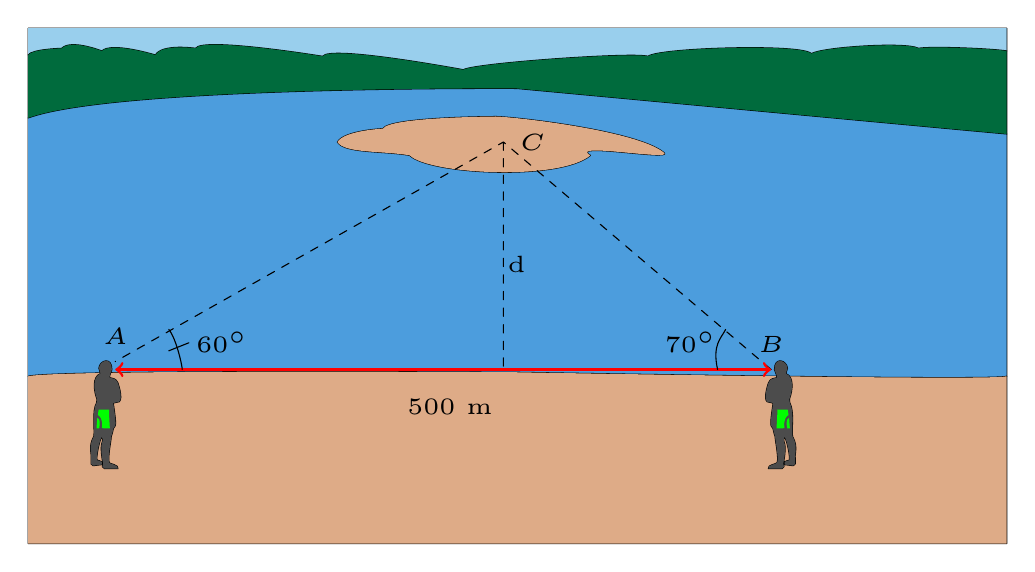
\begin{tikzpicture}[line join=round, line cap=round,scale=1.7,transform shape]			
			\tikzset{dao/.pic={
					\def\H{ 
						(-1.34,1.1)
						..controls +(60:.1) and +(-160:0) .. (-1,1.2)
						..controls +(60:.1) and +(140:0) .. (-.18,1.29)
						..controls +(10:.06) and +(140:0.27) .. (1.1,1.02)
						..controls +(-40:.1) and +(150:0.2) .. (.55,1)
						..controls +(-140:.3) and +(-45:0.2) .. (-.8,1)
						..controls +(170:.2) and +(-60:0.1) .. cycle
						;}
					\draw \H;
					\fill[tumbleweed] \H;
			}}
			\tikzset{nui/.pic={
					\def\T{ %Trời
						(-3.65,1.75)
						..controls +(60:.05) and +(-160:0) .. (-3.4,1.8)
						..controls +(45:.1) and +(-150:0) .. (-3.1,1.78)
						..controls +(45:.1) and +(-150:0) .. (-2.7,1.75)
						..controls +(60:.1) and +(-160:0) .. (-2.4,1.8)
						..controls +(60:.1) and +(-160:0) .. (-1.45,1.74)
						..controls +(60:.1) and +(-160:0) .. (-.4,1.64)
						..controls +(30:.1) and +(160:0.1) .. (.98,1.74)
						..controls +(40:.1) and +(130:0.1) .. (2.2,1.76)
						..controls +(30:.1) and +(150:0.1) .. (3,1.8)
						..controls +(10:.1) and +(170:0.1) .. (3.66,1.78)--(3.66,1.95)--(-3.65,1.95)--cycle
						;}
					\draw \T;
					\fill[lightcornflowerblue] \T;
					\def\N{ 
						(-3.65,1.75)
						..controls +(60:.05) and +(-160:0) .. (-3.4,1.8)
						..controls +(45:.1) and +(-150:0) .. (-3.1,1.78)
						..controls +(45:.1) and +(-150:0) .. (-2.7,1.75)
						..controls +(60:.1) and +(-160:0) .. (-2.4,1.8)
						..controls +(60:.1) and +(-160:0) .. (-1.45,1.74)
						..controls +(60:.1) and +(-160:0) .. (-.4,1.64)
						..controls +(30:.1) and +(160:0.1) .. (.98,1.74)
						..controls +(40:.1) and +(130:0.1) .. (2.2,1.76)
						..controls +(30:.1) and +(150:0.1) .. (3,1.8)
						..controls +(10:.1) and +(170:0.1) .. (3.66,1.78)--(3.66,1.16)
						..controls +(175:.2) and +(20:0) .. (0,1.5)
						..controls +(20:0) and +(20:.7) .. (-3.65,1.28)--cycle
						;}
					\draw \N;
					\fill[cadmiumgreen] \N;
			}}			
			\tikzset{bien/.pic={
					\def\B{ 
						(3.66,1.16)
						..controls +(175:.2) and +(20:0) .. (0,1.5)
						..controls +(20:0) and +(20:.7) .. (-3.65,1.28)--(-3.65,-.65)
						..controls +(15:.2) and +(120:0) .. (0,-.62)
						..controls +(-60:0) and +(-160:0.1) .. (3.66,-.65)--(3.66,1.16)
						;}
					\draw \B;
					\fill[trueblue!70!] \B;
					\def\C{ %Cát
						(-3.65,-.65)
						..controls +(15:.2) and +(120:0) .. (0,-.62)
						..controls +(-60:0) and +(-160:0.1) .. (3.66,-.65)--(3.66,-1.9)--(-3.65,-1.9)--cycle
						;}
					\draw \C;
					\fill[tumbleweed] \C;
			}}			
			\tikzset{nguoi/.pic={
					\def\N{ 
						(-3.04,-.64)--(-3.025,-.6)
						..controls +(90:.1) and +(85:0.06) .. (-3.122,-.59)--(-3.11,-.63)
						..controls +(-160:.07) and +(110:0.05) .. (-3.14,-.81)
						..controls +(-40:.01) and +(60:0) .. (-3.14,-.85)
						..controls +(-120:.07) and +(80:0.05) .. (-3.16,-1.1)
						..controls +(-120:.09) and +(80:0.05) .. (-3.18,-1.28)
						..controls +(-120:.02) and +(170:0.01) .. (-3.165,-1.318)--(-3.1,-1.31)--(-3.1,-1.29)
						..controls +(120:.01) and +(-30:0) .. (-3.135,-1.278)
						..controls +(120:.02) and +(-120:0.04) .. (-3.1,-1.1)
						..controls +(-70:.04) and +(120:0.01) ..(-3.096,-1.14)
						..controls +(-120:.04) and +(120:0.01) ..(-3.09,-1.3)
						..controls +(-120:.02) and +(170:0.02) .. (-3.08,-1.34)--(-2.98,-1.34)
						..controls +(70:.03) and +(-70:0.01) .. (-3.045,-1.296)
						..controls +(110:.04) and +(-70:0.01) .. (-3.03,-1.1)
						..controls +(70:.03) and +(-100:0.01) .. (-3.014,-1.04)--(-3,-1.02)
						..controls +(70:.03) and +(-100:0.01) .. (-3.014,-.85)--(-2.97,-.84)
						..controls +(40:.04) and +(-10:0) .. (-2.98,-.7)
						..controls +(110:.04) and +(-20:0.02) .. (-3.043,-.66)--cycle
						;}
					\draw \N;
					\fill[black!70!] \N;
					\def\Q{ %quần
						(-3.045,-.9)
						..controls +(120:.01) and +(-30:0) .. (-3.04,-1.04)
						-- (-3.1,-1.038)
						..controls +(80:.07) and +(-10:0.01) .. (-3.13,-.94)--(-3.124,-.9)--cycle
						(-3.14,-1.04)--(-3.12,-1.04)
						..controls +(80:.07) and +(-10:0.01) .. (-3.134,-.96)--cycle
						;}
					%\draw \Q;
					\fill[green] \Q;					
			}}			
			\path
			(0,0)pic[scale=1]{bien} (0,0)pic[scale=1]{dao}
			(0,0)pic[scale=1]{nui}
			(0,0)pic[scale=1]{nguoi} (-1.1,0)pic[scale=1,rotate=180,yscale=-1]{nguoi}
			;			
			\draw[dashed] (1.9,-.6) node[above] {\tiny $B$}--(-.1,1.1)node[right] {\tiny $C$}--(-3,-.54)node[above] {\tiny $A$} (-.1,1.1)--(-.1,-.6);
			\draw (-2.6,-.46)--(-2.45,-.4);%gạch góc
			\draw[<->,red,line width=1] (-3,-.6)--(1.9,-.6);
			\node at (-.5,-.7) [below]{\tiny $500$ m};
			\node at (0,0) [above]{\tiny d};
			\node at (-2.2,-.6) [above]{\tiny $60^\circ$};
			\node at (1.3,-.6) [above]{\tiny $70^\circ$};
			%góc
			\draw (-2.6,-.3)
			..controls +(-50:.09) and +(60:0.01) .. (-2.5,-.6);
			\draw[scale=1,rotate=180,xscale=.6,yscale=-1] (-2.6,-.3)
			..controls +(-50:.09) and +(70:.2) .. (-2.5,-.6);
		\end{tikzpicture}
	\end{center}	
	\shortans{$531$}
	\loigiai{Gọi hình chiếu của mép hòn đảo tới bờ biển là $H$. \\ 
		Khi đó các tam giác $CAH$ và $CBH$ vuông tại $H$ nên $\heva{&\tan \widehat{CAH}=\dfrac{CH}{AH} \\& \tan \widehat{CBH}=\dfrac{CH}{BH}}\Rightarrow \heva{&AH=\dfrac{CH}{\tan \widehat{CAH}} \\ &BH=\dfrac{CH}{\tan \widehat{CBH}}.}$\\
		Từ đó ta có $AB=AH+BH=\dfrac{CH}{\tan \widehat{CAH}}+\dfrac{CH}{\tan \widehat{CBH}}=CH\left(\dfrac{1}{\tan \widehat{CAH}}+\dfrac{1}{\tan \widehat{CBH}}\right)$.\\
		Từ đó ta có ngay $CH=\dfrac{AB}{\dfrac{1}{\tan \widehat{CAH}}+\dfrac{1}{\tan \widehat{CBH}}}=\dfrac{500}{\dfrac{1}{\tan 60^\circ}+\dfrac{1}{\tan 70^\circ}}\approx 531$\,(m).		
	}	
\end{ex}
\Closesolutionfile{ans}
% \begin{indapan}
% 	{ans/0-HK1-KN-3-DoanThiDiem-HaNoi-2324}
% \end{indapan}